%!TEX root=C:/Users/Sergej/Documents/GitHub/Thesis/main.tex
\section{Ranking of structural Ricardian comparative advantage }
In this section I present the results of the structural RCA ranking for both value-added exports measures and gross exports.
I show two applications about the structural RCA ranking.
First, I show a scatter plot of the association of the RCA ranking for gross exports and value-added exports and a country's GDP per capita.
This application analysis the hypothesis that countries with a higher GDP show a higher similarity between the rankings.
The reason may be that more developed countries have less sector specific factor usage in the production. \par
The second application compares the structural RCA ranking for Belgium and Germany based on forward and backward value-added exports and gross exports.
By analysing the pattern of RCA for a country pair, it can be directly seen whether value-added exports change the conclusions about a countries comparative advantage.
Moreover, I research whether both perspectives show a similar story about a countries comparative advantage industries.
\subsection{Structural Ricardian comparative advantage based gross exports and value-added exports}
To compare the RCA rankings I have chosen the following association.
First of all, I chose the Spearman's $\rho$  since I focus on the similarity of the rankings.
Moreover I chose Kendall's $\tau$ as it computes the similarity of the two rankings, by counting the number of country pairs, which are different between two rankings.
In addition, Kendall's  $\tau$ may be interpreted as the difference between the probability of concordance and disconcordance of two variables \parcite{newson2parameters}.
\par &
% I outline the construction of Kendall's $\tau$ based on \textcite{abdi2007kendall}.
% The outline makes the simple interpretation of Kendall's $\tau$ in terms of probabilities more clear.
% The basic idea behind the measure is to count the number of different pairs of two sets of ordered  objects, which include the same objects  \textcite{abdi2007kendall}.
% I illustrate this idea in the context of the RCA rankings.
% For two RCA rankings, the measure is based on counting the number of different ordered country pairs, which I denote as $d(P_1, P_2)$, where $P_i \quad i=1,2$ indicates the two ordered set of pairs obtained from the country rankings.
% In the next step, this number is normalized such that is bounded by -1 and 1, where -1 reflects the largest differences and 1 is equal to the smallest difference.
% Kendall's $\tau$ is then defined as follows \[ \tau= \frac{1/2 N(N-1) - d(P_1,P_2)} {1/2 N(N-1)} .\] %where the nominator $1/2 N(N-1)$ is equal to the number of pairs one can obtain from a set of $n$ objects.
% Moreover, Kendall's $\tau$ has an intuitive stochastic interpretation based on the idea of drawing ordered pairs \parencite{abdi2007kendall}.
% In the context of two country rankings, the interpretation is that if a country pair is randomly drawn from each ranking, Kendall's $\tau$ is the difference between the probability that the draws have the same order and the probability that the country pairs have a different order.
% The focus of Kendall's $\tau$ on country pairs is especially useful for RCA, as the main focus of RCA is to compare pairs of countries and industries.   \par
\begin{figure}[H]
\caption{Association RCA based on VAX \& EXGR and GDP per capita }
\centering
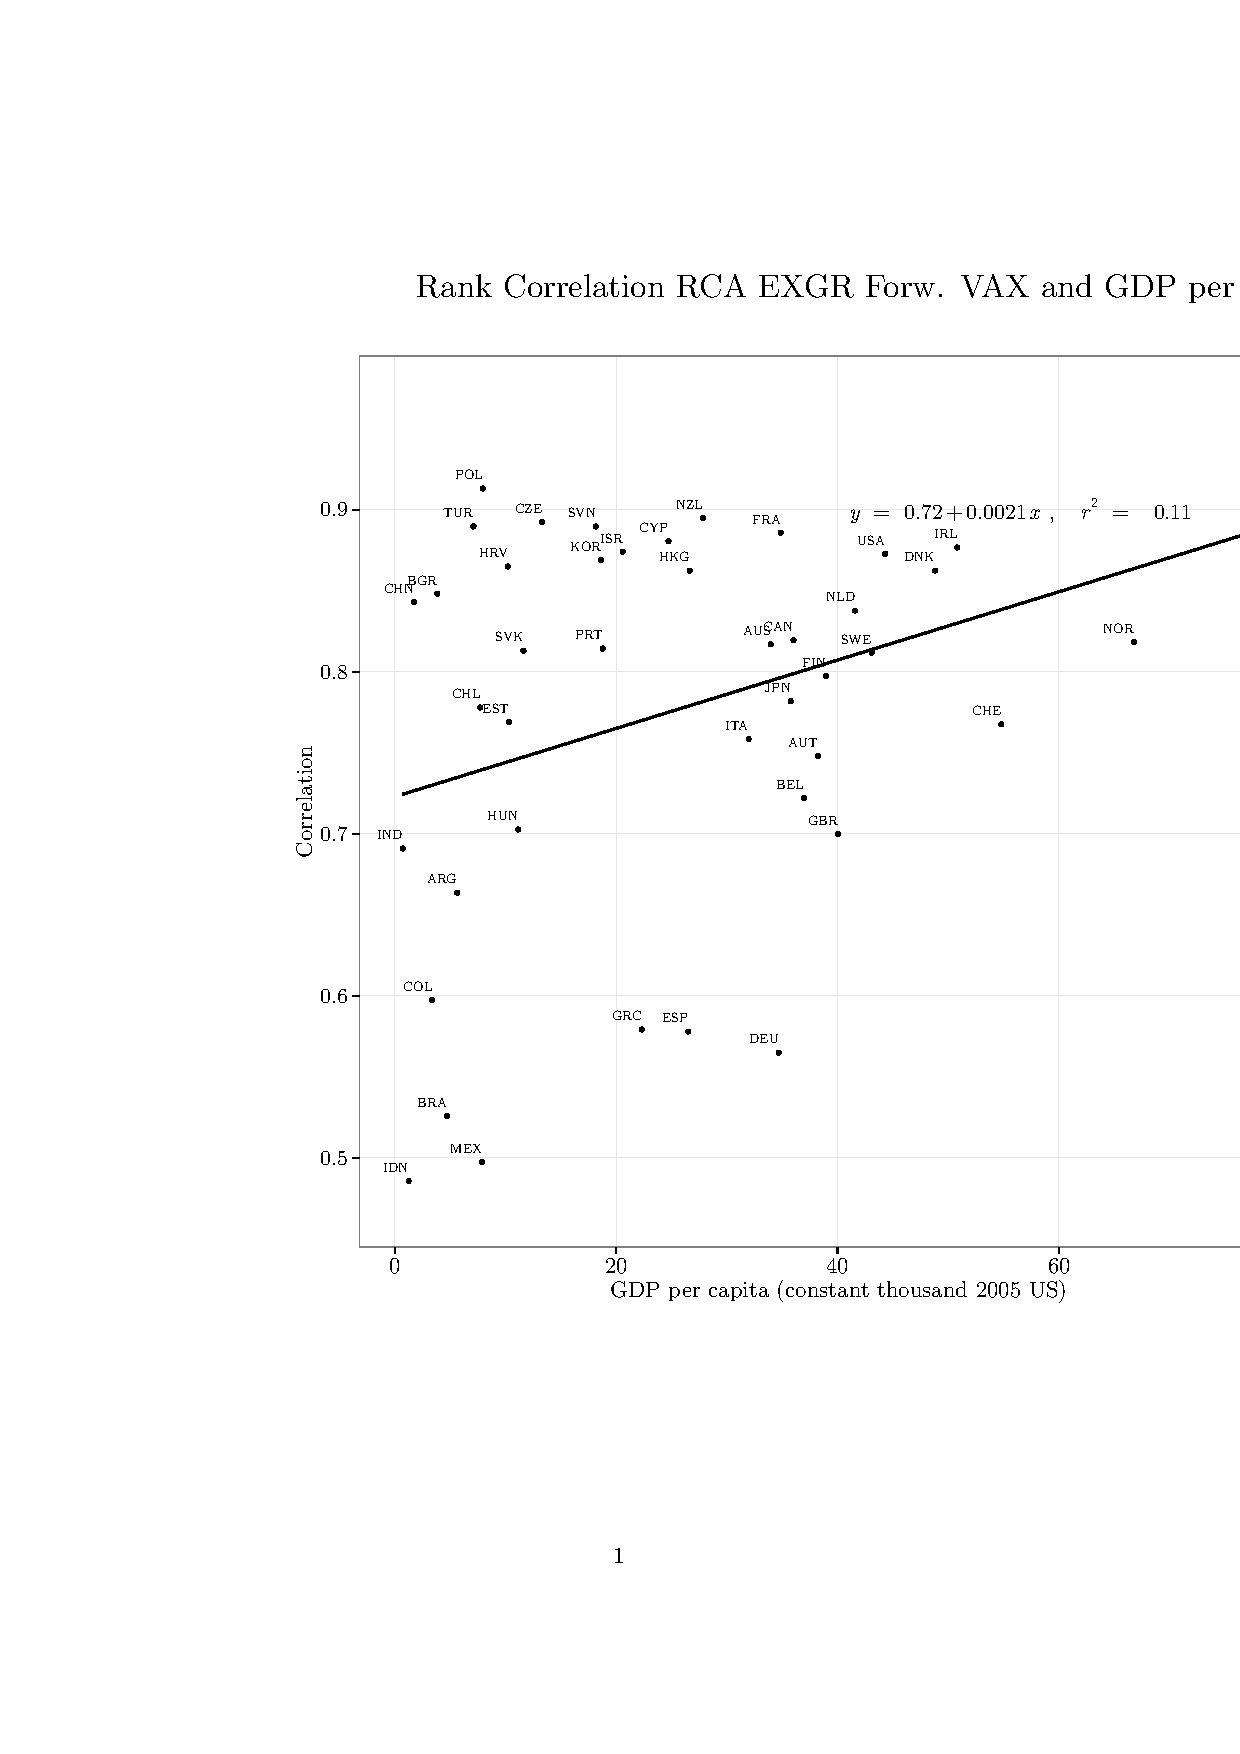
\includegraphics[width=.49 \linewidth]{./fig/spearman_fddva_std_balassa-march.tex}
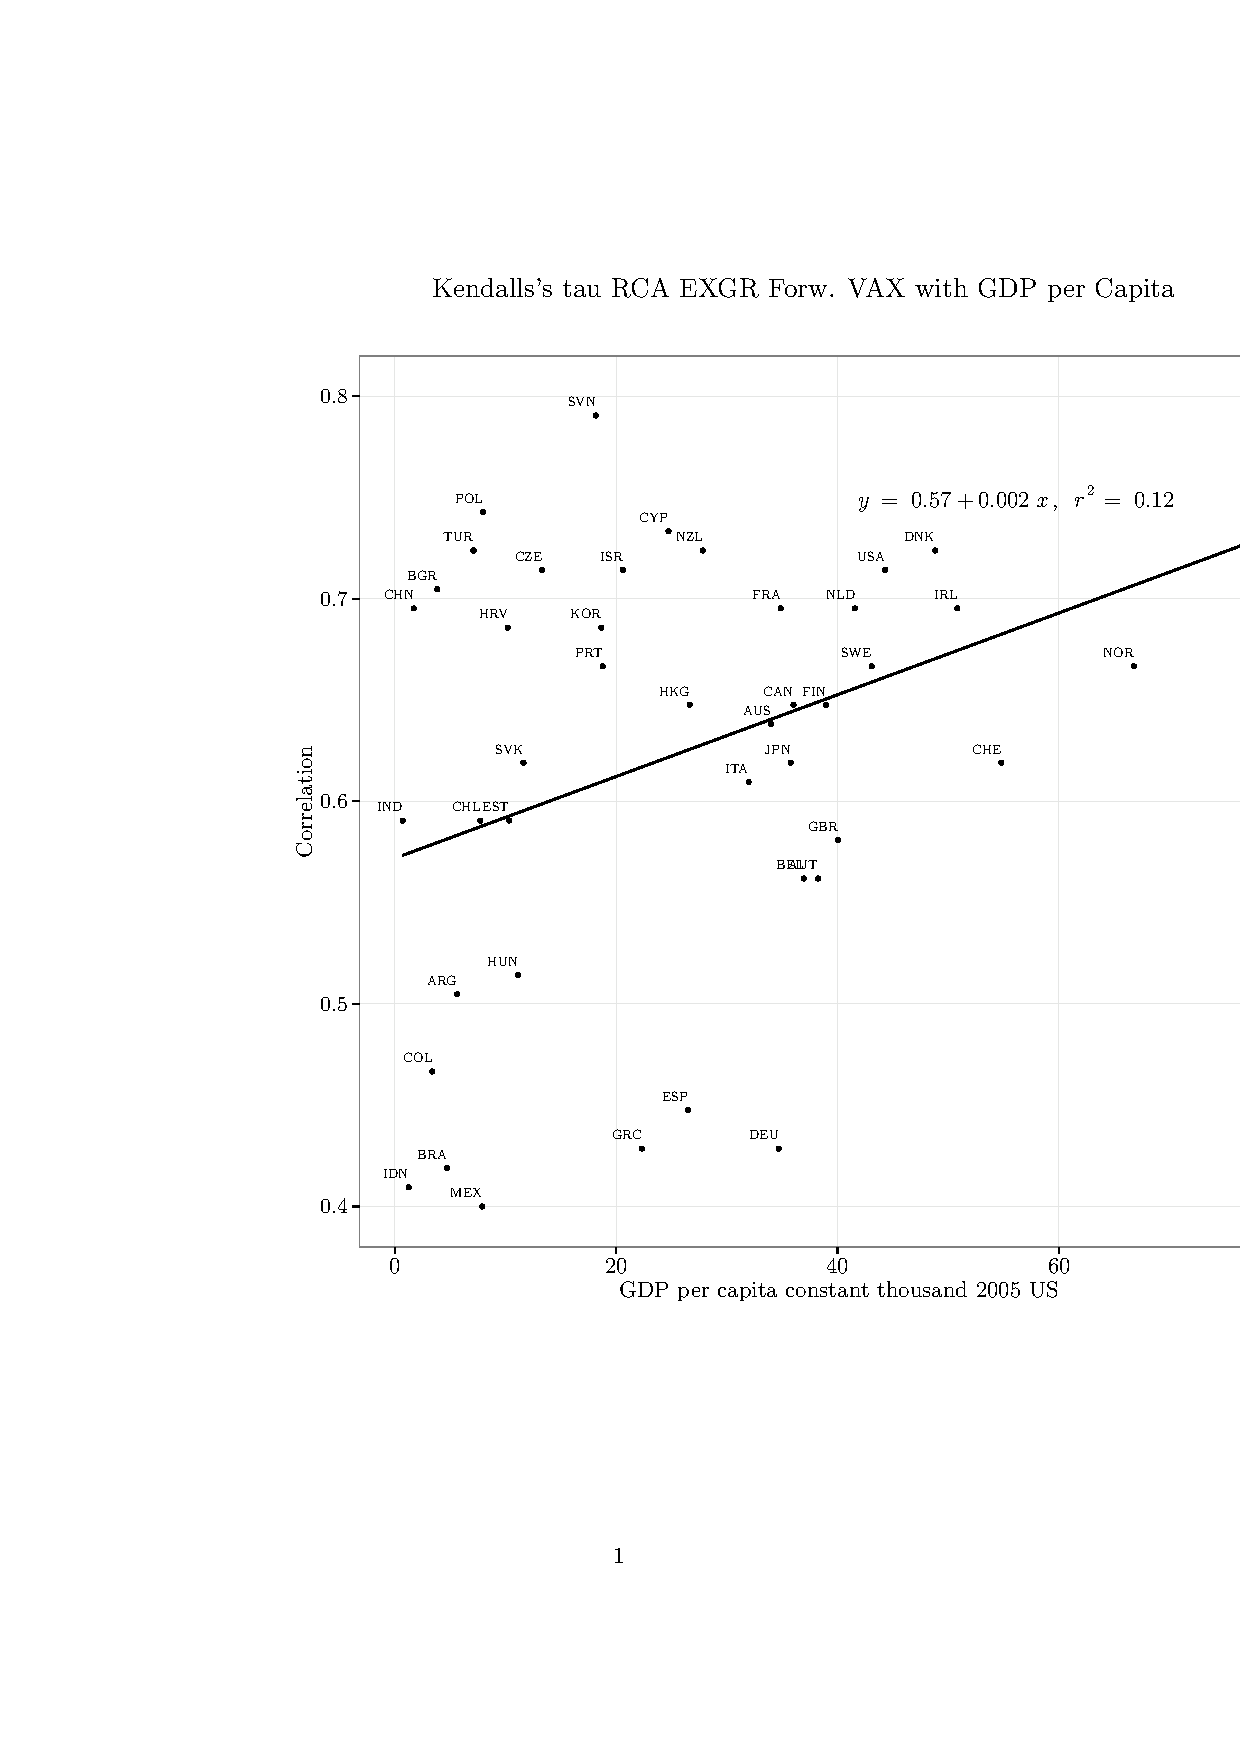
\includegraphics[width=.49\linewidth]{./fig/kendall_fddva_exgr_std_balassa-march.tex}
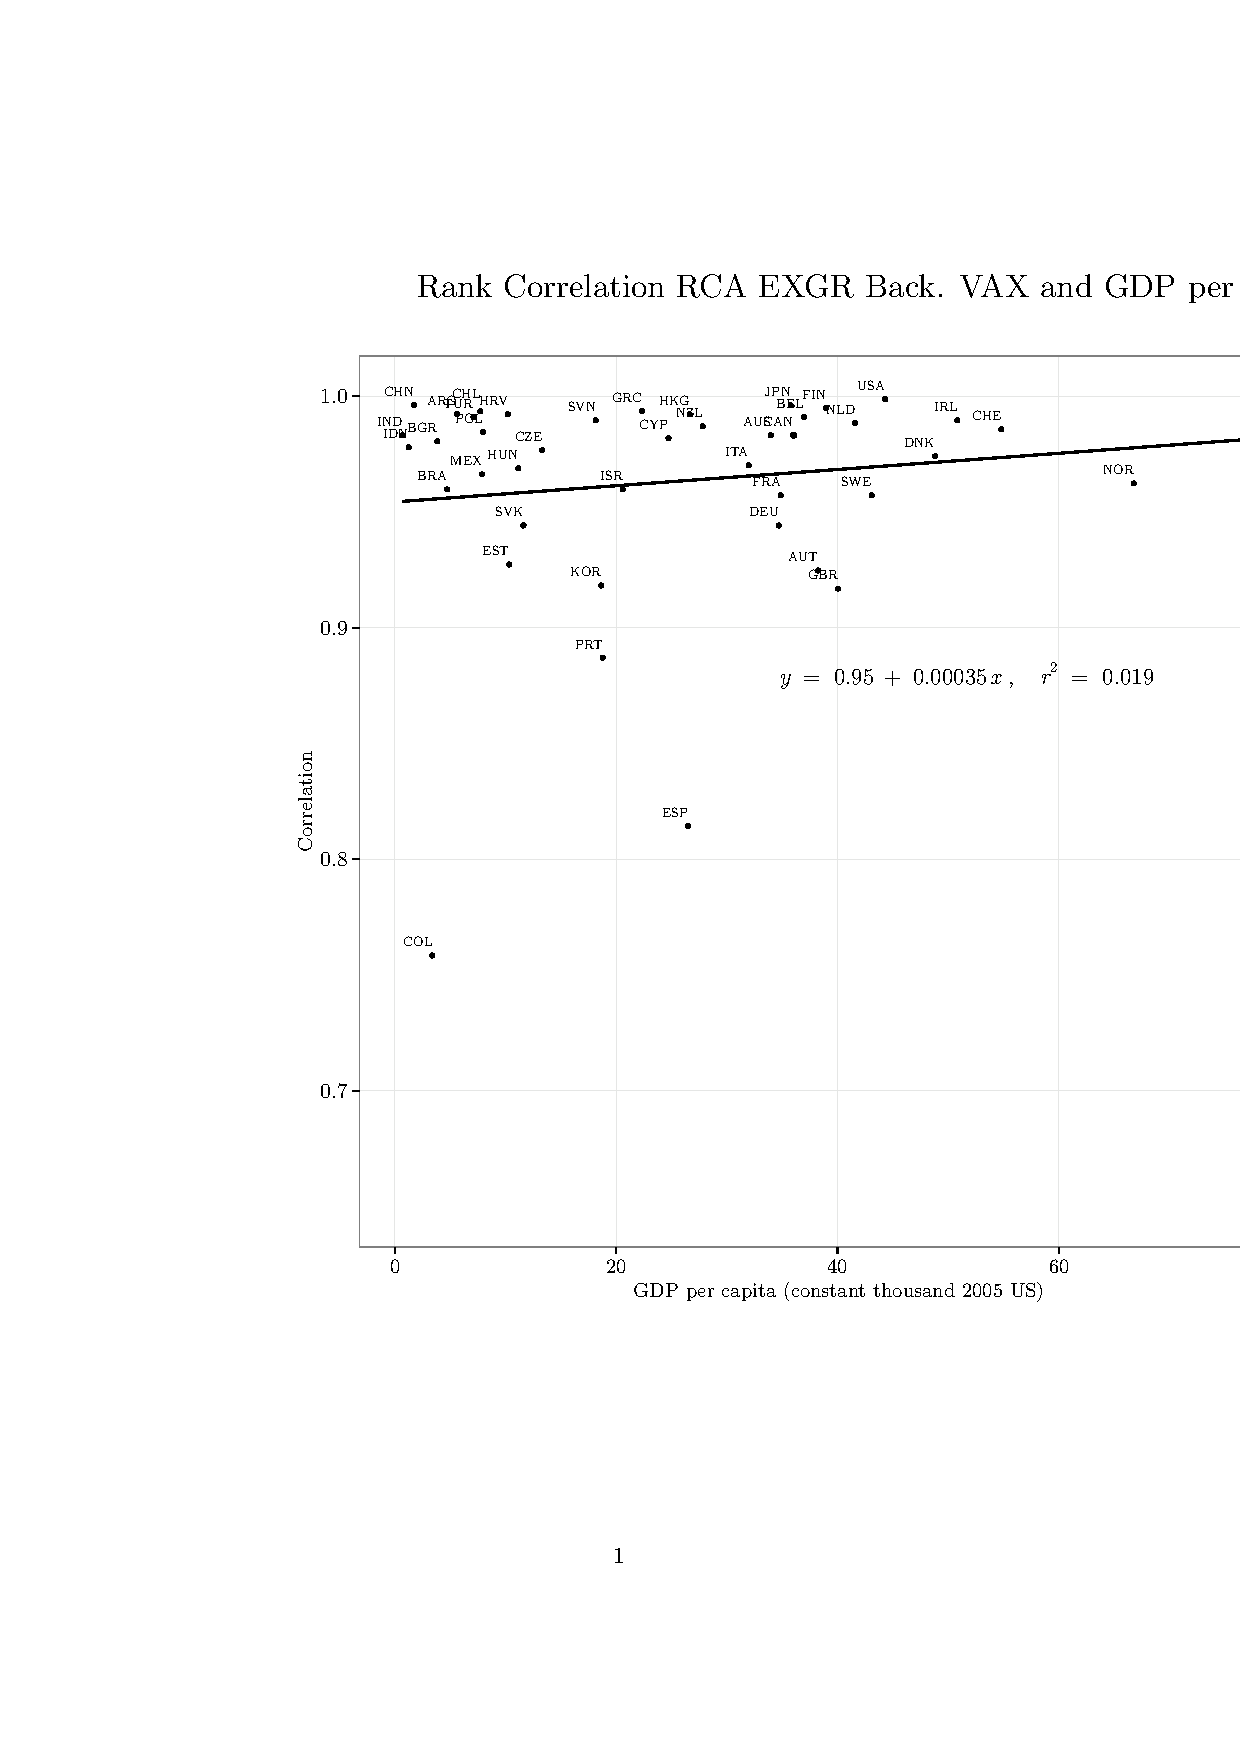
\includegraphics[width=.49 \linewidth]{./fig/spearman_exgr_dva_std_balassa-march.tex}
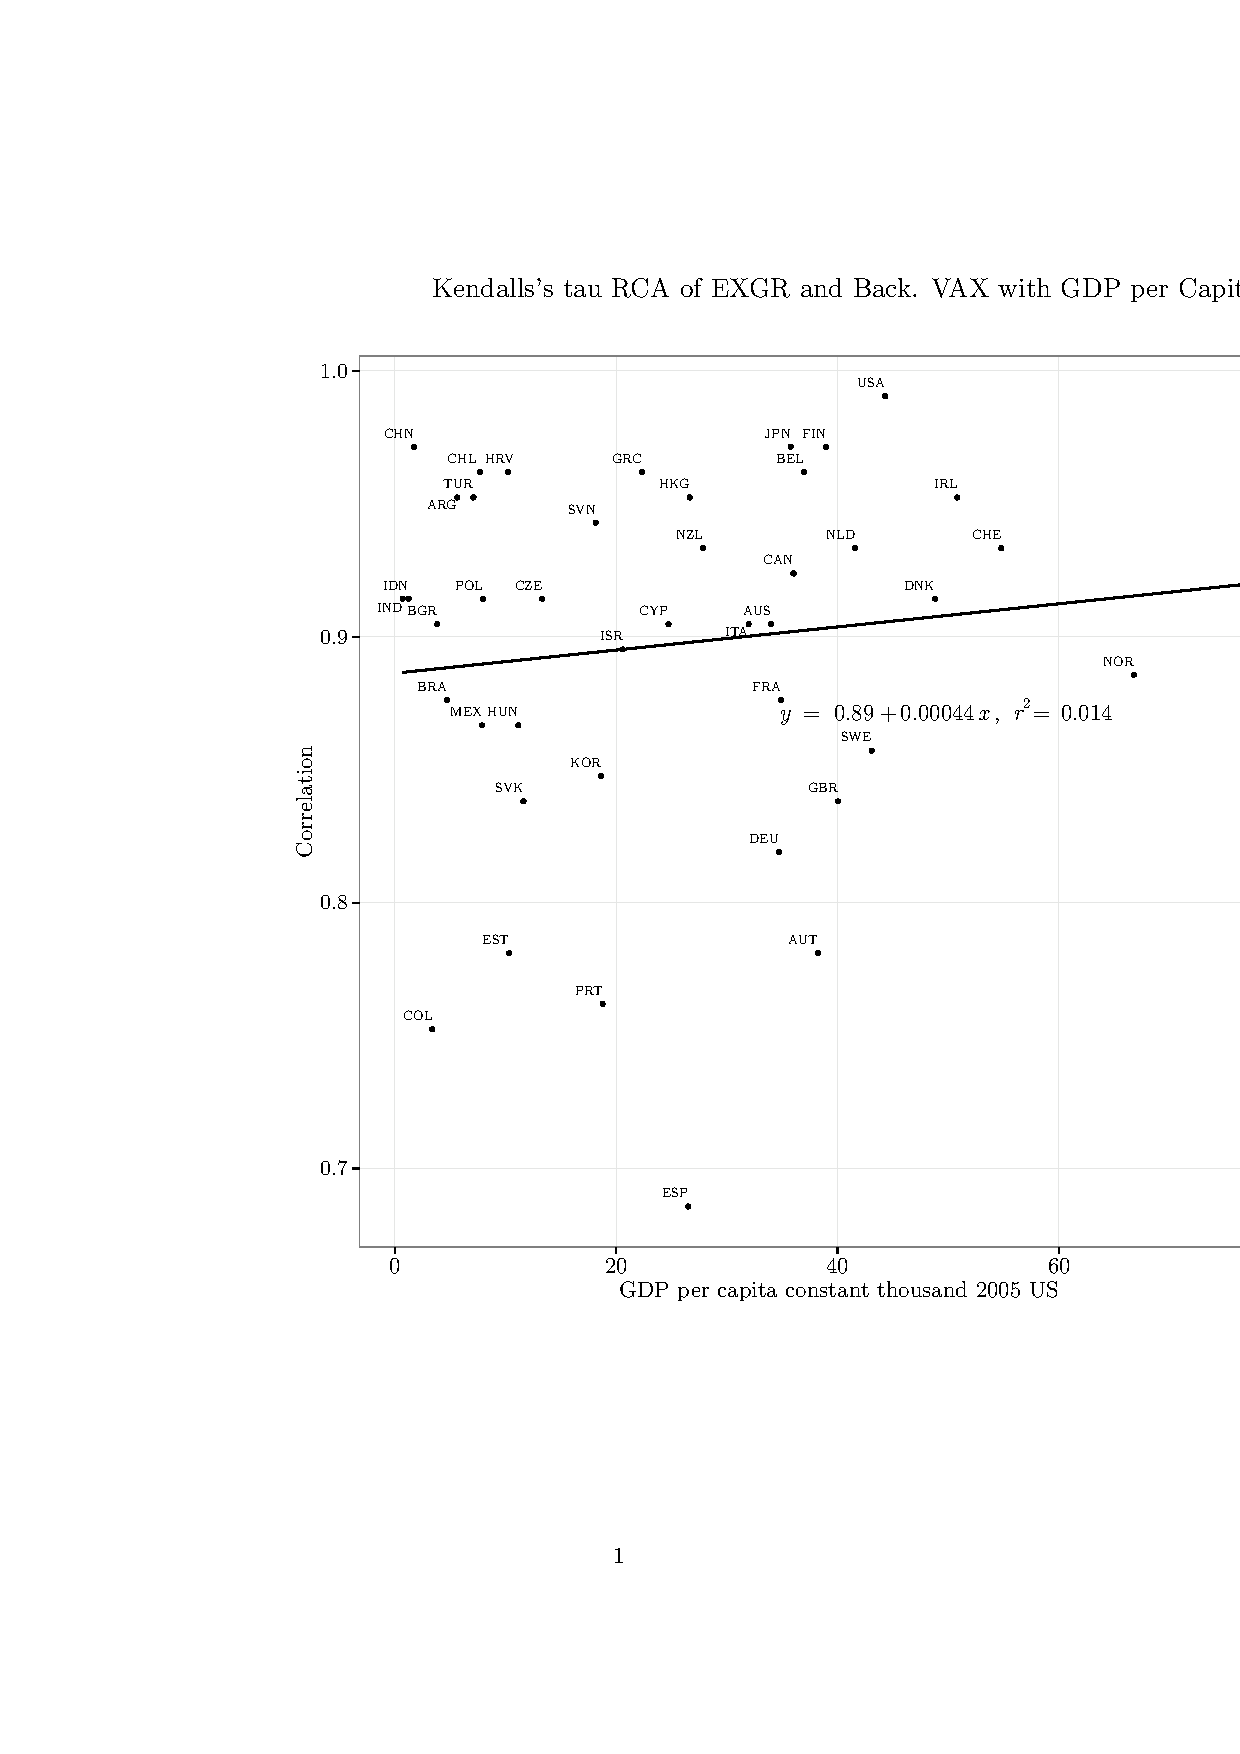
\includegraphics[width=.49\linewidth]{./fig/kendall_dva_exgr_std_balassa-march.tex}
 %\captionof{figure}{Another figure}
\end{figure}
I conclude four findings from the figures above.
Firstly, the RCA rankings based on gross exports and backward value-added exports show a high degree of similarity for all countries.
Secondly, the association between forward value-added exports and gross exports is substantially lower than the association of backward value-added and gross exports.
Thirdly,  the association of gross exports and forw. VAX show a weak positive association with a country's GDP per capita.
However the positive relation in the graph is not robust, as the exclusion of the country with the lowest and the highest  .
As a final point I find that the overall strength of the associations is higher using  Spearman's $\rho$ compared to Kendall's $\tau$. \par
The first and second finding are similar to the results in the estimation of the $\theta$ parameter, which showed similar estimates using gross exports and backward value-added exports while the estimates using forw. VAX showed differences.
The third finding is consistent with the hypothesis   that countries with a higher GDP have less sector specific input and sourcing patterns.
The finding of a smaller association for Kendall compared to Spearman is unsprising, given that the population analog of Spearman's $\rho$ and Kendall's $\tau$ is equal to three half \parencite{fredricks2007}. \par
The country pair graph comparing RCA for the three indicators backward/forward value-added exports and gross exports present a more local view of RCA.
 below I present  the normalized RCA based on both value-added export measures and gross exports for the industries of the manufacturing sector.
the RCA \footnote{ Formally, I define it as follows $RCA_{i}^{k}=\frac{ z^k_i * \bar{z} }{\bar{z}_i * \bar{z}^k}$, where $\bar{z}=1/NK* \sum_{i=1}^N \sum_{k=1}^K z^k_i$ denotes the grand mean, $\bar{z}^k= 1/N \sum_{i=1}^N z^k_i$ denotes the industry specific mean and $\bar{z}_i= 1/K \sum_{k=1}^K z^k_i$ denotes the country specific mean.} as in \textcite{leromain2014}.
The normalized RCA has the following interpretation, a value above (below) 1 indicates a comparative (dis)advantage of a country in a specific industry.
 \par
To start with the RCA ranking results, I discuss the results for backward value-added exports and gross exports.
I find that for both countries backward value added closely traces the RCA pattern of gross exports.
This results resembles the result of the estimation of $\theta$, where I observed a similar pattern. \par
The graph highlights that both countries highlights have an comparative advantage in the following sectors 20 23 24 26.
Germany has an higher comparative advantage in seven industries namely 20 21-22 25 27-28 29 30-33 34-35.
On the other hand, Belgium has an comparative advantage in six industries namely the food industry, 17-19 23 24 26 36-37.
 \par
In contrast, I observe that the RCA rankings are different for forward value-added gross exports.
The largest decrease of RCA based on forw. value-added exports compared to gross exports is in the industries 23 and 20.
Additionally for Germany large decrease of RCA for the industry 21-22.
The largest decrease of RCA induces a change of 15\%  in the industry 23 for both countries.
As a result, the industry 23 changes from a comparative advantage to a comparative disadvantage for Germany.
The industry changes from an comparative advantage to comparative disadvantage, whereas for Belgium the industry remains a comparative advantage.
Additionally, in industry 20 both countries show no longer an comparative advantage under forw. VAX, whereas under gross exports they show an comparative advantage.
Moreover, I observe the largest increase of RCA under VAX compared to EXGR in the industry 29 and 30-33.
For both countries I observe an increase of about 5\% in the industry 30-33 for forw. VAX, and a somewhat smaller increase in the industry 29.
However, the pattern of RCA remains unchanged for both countries, for Belgium an comparative disadvantage and Germany has an comparative advantage.
Concluding, the graphs show that forward value-added exports changes the pattern of RCA, whereas backward value-added exports traces the pattern of RCA under gross exports.
 \begin{figure}
\caption{Country pair RCA based on for- and backward  VAX \& EXGR }
\includegraphics[width=.5\linewidth]{./fig/forw_exgr_DEU_BEL_tiva.tex}
\includegraphics[width=.5\linewidth]{./fig/back_exgr_DEU_BEL_tiva.tex}
\end{figure}

\subsection{RCA based on WIOD}
In this subsection I compare the previous results about the RCA for BEL and GER to the results based on the WIOD data.
Firstly, compared to the TiVA data the WIOD data comes at a greater level of dissagregation.
\begin{figure}
\caption{Country pair RCA based on for- and backward  VAX \& EXGR }
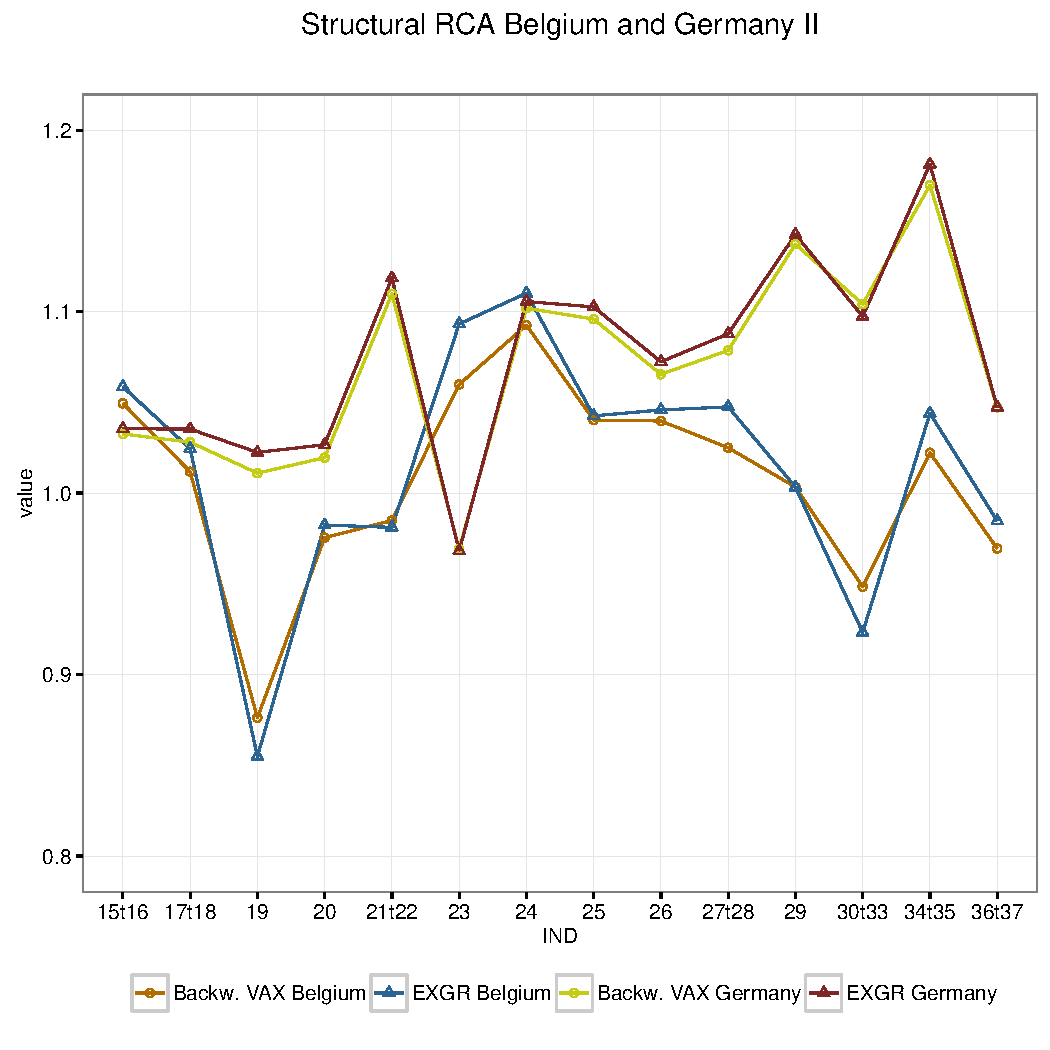
\includegraphics[width=.5\linewidth]{./fig/back_exgr_DEU_BEL_wiod.pdf}
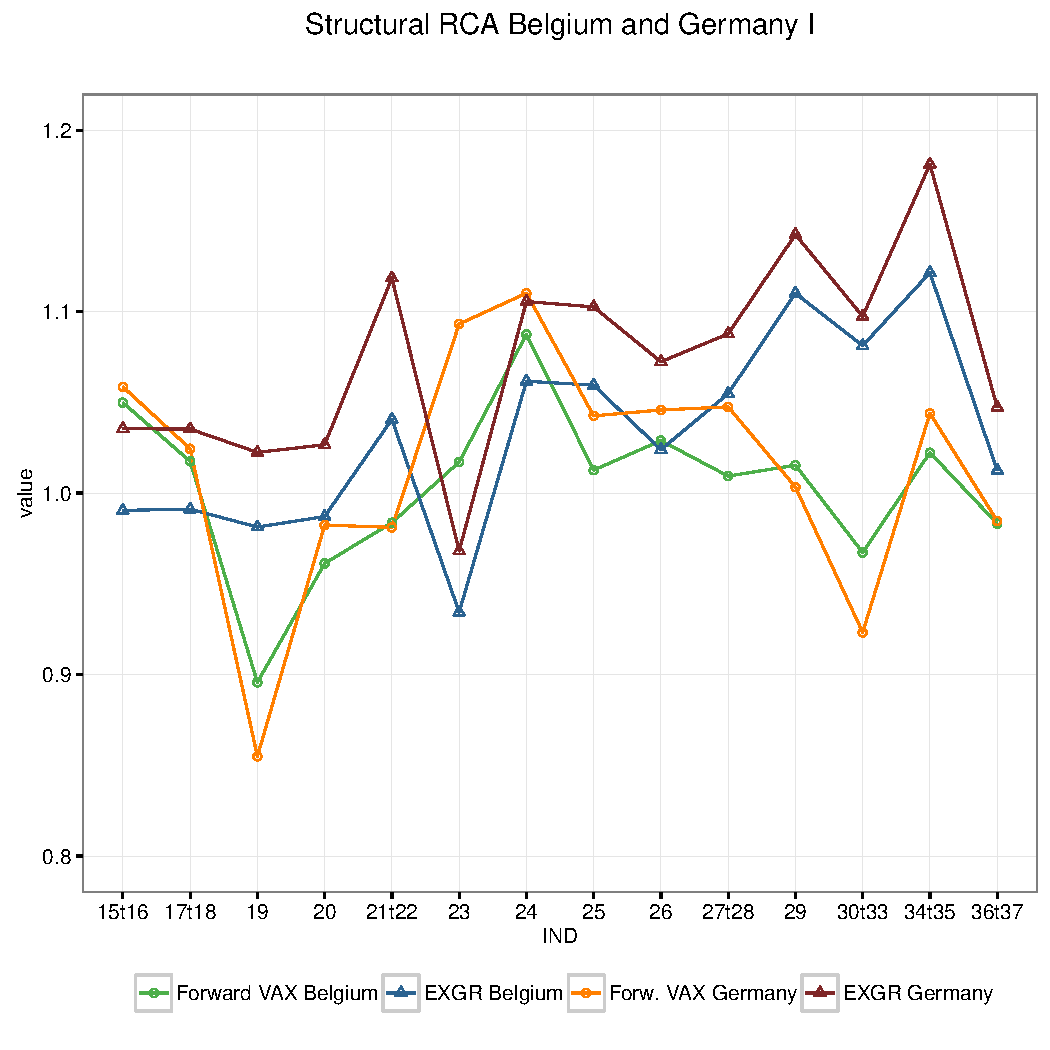
\includegraphics[width=.5\linewidth]{./fig/forw_exgr_DEU_BEL_wiod.pdf}
\end{figure}
\endinput
